\documentclass{article}
\usepackage[utf8]{inputenc}

% Essential packages for article format
\usepackage{amsmath, amssymb, amsfonts}
\usepackage{bm}
\usepackage{graphicx}
\usepackage{xcolor}
\usepackage{tcolorbox}
\usepackage[bookmarks=false]{hyperref}
\usepackage{url}
\usepackage{booktabs}
\usepackage{array}
\usepackage{multirow}
\usepackage{enumitem}
\usepackage{tikz}
\usetikzlibrary{arrows.meta, positioning, shapes.geometric, trees}

% Additional packages for a nice tutorial format
\usepackage[margin=1in]{geometry}
\usepackage{fancyhdr}
\usepackage{titlesec}

% Header and footer setup
\pagestyle{fancy}
\fancyhf{}
\rhead{Tutorial: Decision Trees}
\lhead{ES335 - Machine Learning}
\rfoot{Page \thepage}

% Title formatting
\titleformat{\section}{\Large\bfseries\color{blue!75!black}}{\thesection}{1em}{}
\titleformat{\subsection}{\large\bfseries\color{blue!60!black}}{\thesubsection}{1em}{}

% Load conventions after math packages
\usepackage{../../shared/styles/conventions}

% Define counters for examples and exercises
\newcounter{example}
\setcounter{example}{0}
\newcounter{exercise}
\setcounter{exercise}{0}

\title{\textbf{Tutorial: Decision Trees} \\ \textit{Building Interpretable Machine Learning Models}}
\author{ES335 - Machine Learning \\ IIT Gandhinagar}
\date{\today}

\begin{document}

\maketitle

\begin{abstract}
Decision trees are among the most intuitive and interpretable machine learning algorithms. This tutorial covers the fundamental concepts, construction algorithms, evaluation metrics, and practical considerations for building effective decision tree models. We'll explore both classification and regression trees, discuss overfitting and pruning strategies, and examine real-world applications through comprehensive examples and exercises.
\end{abstract}

\tableofcontents
\newpage

\section{Introduction: Why Decision Trees?}

Imagine you're a doctor diagnosing a patient. You might ask:
\begin{itemize}
    \item Is the patient's temperature above 38°C?
    \item If yes, does the patient have a cough?
    \item If yes to both, does the patient have difficulty breathing?
\end{itemize}

This logical sequence of questions forms a \textbf{decision tree} - a flowchart-like structure that makes decisions by asking a series of questions about the input features.

\begin{center}
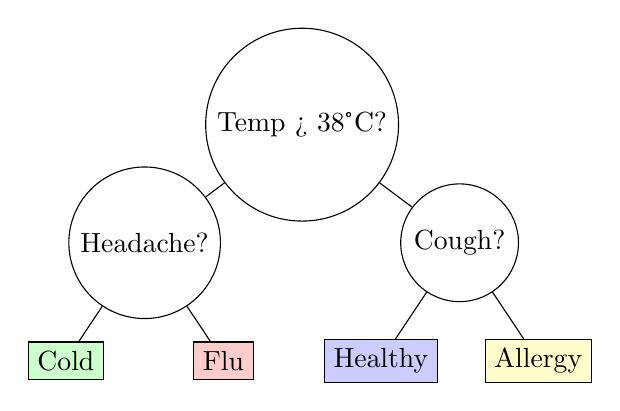
\begin{tikzpicture}[
  level distance=1.5cm,
  level 1/.style={sibling distance=4cm},
  level 2/.style={sibling distance=2cm},
  level 3/.style={sibling distance=1.5cm}
]
\node [circle, draw] {Temp > 38°C?}
  child {node [circle, draw] {Headache?}
    child {node [rectangle, draw, fill=green!20] {Cold}}
    child {node [rectangle, draw, fill=red!20] {Flu}}
  }
  child {node [circle, draw] {Cough?}
    child {node [rectangle, draw, fill=blue!20] {Healthy}}
    child {node [rectangle, draw, fill=yellow!20] {Allergy}}
  };
\end{tikzpicture}
\end{center}

\textbf{Key Advantages}:
\begin{itemize}
    \item \textbf{Interpretability}: Easy to understand and explain
    \item \textbf{No assumptions}: Works with any data distribution
    \item \textbf{Mixed data types}: Handles categorical and numerical features
    \item \textbf{Feature selection}: Automatically identifies important features
    \item \textbf{Non-linear patterns}: Captures complex relationships
\end{itemize}

\section{Mathematical Foundation}

\subsection{Information Theory Basics}

Decision trees work by asking questions that \textbf{reduce uncertainty}. We measure uncertainty using information theory concepts.

\textbf{Entropy} measures the "impurity" or uncertainty in a dataset:
$$H(S) = -\sum_{i=1}^c p_i \log_2(p_i)$$

where $p_i$ is the proportion of samples belonging to class $i$.

\begin{tcolorbox}[colback=blue!5!white,colframe=blue!75!black,title=Example \stepcounter{example}\#\theexample: Calculating Entropy]
Dataset with 8 positive and 2 negative examples:
$$p_+ = \frac{8}{10} = 0.8, \quad p_- = \frac{2}{10} = 0.2$$
$$H(S) = -0.8 \log_2(0.8) - 0.2 \log_2(0.2) = -0.8(-0.322) - 0.2(-2.322) = 0.722$$

High entropy (close to 1) means high uncertainty, low entropy (close to 0) means low uncertainty.
\end{tcolorbox}

\textbf{Information Gain} measures how much a feature reduces entropy:
$$\text{Gain}(S, A) = H(S) - \sum_{v \in \text{Values}(A)} \frac{|S_v|}{|S|} H(S_v)$$

where $S_v$ is the subset of $S$ where feature $A$ has value $v$.

\subsection{Decision Tree Construction Algorithm}

The \textbf{ID3 algorithm} builds trees by recursively selecting the feature with highest information gain:

\begin{enumerate}
    \item Calculate entropy of current dataset $S$
    \item For each feature $A$:
    \begin{itemize}
        \item Split dataset based on feature values
        \item Calculate weighted average entropy of splits
        \item Compute information gain
    \end{itemize}
    \item Select feature with maximum information gain
    \item Create child nodes for each feature value
    \item Recursively apply to each child node
    \item Stop when: pure node, no more features, or minimum samples reached
\end{enumerate}

\begin{tcolorbox}[colback=green!5!white,colframe=green!75!black,title=Example \stepcounter{example}\#\theexample: Building a Tree Step by Step]

\textbf{Tennis Dataset}: Play tennis based on weather conditions.

\begin{center}
\begin{tabular}{|c|c|c|c|c|}
\hline
\textbf{Outlook} & \textbf{Temperature} & \textbf{Humidity} & \textbf{Wind} & \textbf{Play?} \\
\hline
Sunny & Hot & High & Weak & No \\
Sunny & Hot & High & Strong & No \\
Overcast & Hot & High & Weak & Yes \\
Rain & Mild & High & Weak & Yes \\
Rain & Cool & Normal & Weak & Yes \\
Rain & Cool & Normal & Strong & No \\
Overcast & Cool & Normal & Strong & Yes \\
Sunny & Mild & High & Weak & No \\
Sunny & Cool & Normal & Weak & Yes \\
Rain & Mild & Normal & Weak & Yes \\
Sunny & Mild & Normal & Strong & Yes \\
Overcast & Mild & High & Strong & Yes \\
Overcast & Hot & Normal & Weak & Yes \\
Rain & Mild & High & Strong & No \\
\hline
\end{tabular}
\end{center}

\textbf{Step 1}: Calculate root entropy
- 9 "Yes", 5 "No" $\rightarrow$ $H(S) = -\frac{9}{14}\log_2(\frac{9}{14}) - \frac{5}{14}\log_2(\frac{5}{14}) = 0.940$

\textbf{Step 2}: Calculate information gain for each feature

For \textbf{Outlook}:
- Sunny: 2 Yes, 3 No $\rightarrow$ $H = 0.971$
- Overcast: 4 Yes, 0 No $\rightarrow$ $H = 0$  
- Rain: 3 Yes, 2 No $\rightarrow$ $H = 0.971$

$$\text{Gain}(Outlook) = 0.940 - [\frac{5}{14} \times 0.971 + \frac{4}{14} \times 0 + \frac{5}{14} \times 0.971] = 0.247$$

\textbf{Result}: Outlook has highest gain $\rightarrow$ becomes root node!
\end{tcolorbox}

\section{Regression Trees}

For continuous target variables, we use \textbf{regression trees} that predict numerical values instead of classes.

\textbf{Key Differences}:
\begin{itemize}
    \item \textbf{Split criterion}: Use variance reduction instead of information gain
    \item \textbf{Leaf values}: Mean of target values in leaf
    \item \textbf{Error measure}: Mean Squared Error (MSE) or Mean Absolute Error (MAE)
\end{itemize}

\textbf{Variance Reduction}:
$$\text{VarReduction}(S, A) = \text{Var}(S) - \sum_{v} \frac{|S_v|}{|S|} \text{Var}(S_v)$$

where $\text{Var}(S) = \frac{1}{n}\sum_{i=1}^n (y_i - \bar{y})^2$

\begin{tcolorbox}[colback=orange!5!white,colframe=orange!75!black,title=Example \stepcounter{example}\#\theexample: Predicting House Prices]

\textbf{Dataset}: House size vs. Price
\begin{center}
\begin{tabular}{|c|c|}
\hline
\textbf{Size (sq ft)} & \textbf{Price (\$k)} \\
\hline
1000 & 150 \\
1200 & 180 \\
1500 & 220 \\
1800 & 280 \\
2000 & 320 \\
2200 & 350 \\
\hline
\end{tabular}
\end{center}

\textbf{Possible split}: Size $\leq$ 1500 vs Size $>$ 1500
- Left: Mean = \$183k, Variance = 1156
- Right: Mean = \$317k, Variance = 1344

This split separates smaller, cheaper houses from larger, expensive ones!
\end{tcolorbox}

\section{Overfitting and Pruning}

\subsection{The Overfitting Problem}

Decision trees can grow very deep and memorize training data, leading to poor generalization.

\begin{center}
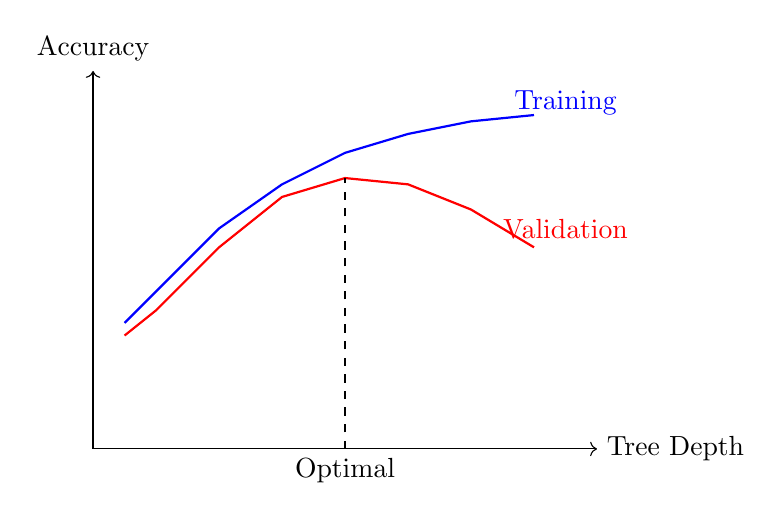
\begin{tikzpicture}[scale=0.8]
    % Training accuracy
    \draw[->] (0,0) -- (8,0) node[right] {Tree Depth};
    \draw[->] (0,0) -- (0,6) node[above] {Accuracy};
    
    % Training curve (always increasing)
    \draw[thick, blue] (0.5,2) -- (1,2.5) -- (2,3.5) -- (3,4.2) -- (4,4.7) -- (5,5.0) -- (6,5.2) -- (7,5.3);
    \node[blue] at (7.5,5.5) {Training};
    
    % Validation curve (increases then decreases)
    \draw[thick, red] (0.5,1.8) -- (1,2.2) -- (2,3.2) -- (3,4.0) -- (4,4.3) -- (5,4.2) -- (6,3.8) -- (7,3.2);
    \node[red] at (7.5,3.5) {Validation};
    
    % Optimal point
    \draw[dashed] (4,0) -- (4,4.3);
    \node[below] at (4,0) {Optimal};
\end{tikzpicture}
\end{center}

\subsection{Pruning Strategies}

\textbf{1. Pre-pruning (Early Stopping)}:
\begin{itemize}
    \item Maximum depth limit
    \item Minimum samples per leaf
    \item Minimum information gain threshold
\end{itemize}

\textbf{2. Post-pruning}:
\begin{itemize}
    \item Build full tree, then remove branches
    \item Use validation set to evaluate pruning
    \item Cost-complexity pruning (minimal cost-complexity)
\end{itemize}

\textbf{Cost-Complexity Pruning}:
$$R_\alpha(T) = R(T) + \alpha |T|$$

where $R(T)$ is the error rate and $|T|$ is the number of leaves. Parameter $\alpha$ controls the trade-off between accuracy and complexity.

\section{Advanced Topics}

\subsection{Handling Categorical Features}

For categorical features with $k$ values, there are $2^{k-1} - 1$ possible binary splits. For large $k$, this becomes computationally expensive.

\textbf{Strategies}:
\begin{itemize}
    \item \textbf{Binary encoding}: Convert categories to binary features
    \item \textbf{Frequency encoding}: Order by target frequency
    \item \textbf{Target encoding}: Use target mean for ordering
\end{itemize}

\subsection{Handling Missing Values}

\textbf{During Training}:
\begin{itemize}
    \item Ignore missing values when calculating information gain
    \item Use probabilistic splits based on observed data
\end{itemize}

\textbf{During Prediction}:
\begin{itemize}
    \item Follow majority path
    \item Use weighted combination of all paths
    \item Surrogate splits (backup features)
\end{itemize}

\subsection{Feature Importance}

Decision trees naturally provide feature importance scores:
$$\text{Importance}(f) = \sum_{t \in \text{splits using } f} p(t) \times \Delta\text{Impurity}(t)$$

where $p(t)$ is the proportion of samples reaching node $t$.

\section{Implementation Considerations}

\subsection{Algorithmic Complexity}

\textbf{Training Time}: $O(n \times m \times \log n)$ where $n$ = samples, $m$ = features
\textbf{Prediction Time}: $O(\log n)$ in balanced tree, $O(n)$ worst case
\textbf{Space Complexity}: $O(n)$ for storing the tree

\subsection{Practical Tips}

\begin{enumerate}
    \item \textbf{Feature scaling}: Not required (trees are scale-invariant)
    \item \textbf{Cross-validation}: Essential for selecting optimal hyperparameters
    \item \textbf{Ensemble methods}: Random Forests and Gradient Boosting improve performance
    \item \textbf{Interpretability vs. accuracy}: Deeper trees are more accurate but less interpretable
\end{enumerate}

\section{Practice Problems}

\subsection{Basic Problems}

\begin{tcolorbox}[colback=gray!5!white,colframe=gray!75!black,title=Problem \stepcounter{exercise}\#\theexercise: Information Gain Calculation]

Given this dataset for predicting "Buy Computer":

\begin{center}
\begin{tabular}{|c|c|c|c|}
\hline
\textbf{Age} & \textbf{Income} & \textbf{Student} & \textbf{Buy?} \\
\hline
Youth & High & No & No \\
Youth & High & No & No \\
Middle & High & No & Yes \\
Senior & Medium & No & Yes \\
Senior & Low & Yes & Yes \\
Senior & Low & Yes & No \\
Middle & Low & Yes & Yes \\
Youth & Medium & No & No \\
Youth & Low & Yes & Yes \\
Senior & Medium & Yes & Yes \\
\hline
\end{tabular}
\end{center}

Calculate the information gain for splitting on "Age".

\textbf{Solution}:
Root entropy: 6 Yes, 4 No $\rightarrow$ $H = -\frac{6}{10}\log_2(\frac{6}{10}) - \frac{4}{10}\log_2(\frac{4}{10}) = 0.971$

Age splits:
- Youth: 1 Yes, 3 No $\rightarrow$ $H = 0.811$
- Middle: 2 Yes, 0 No $\rightarrow$ $H = 0$
- Senior: 3 Yes, 1 No $\rightarrow$ $H = 0.811$

$\text{Gain}(Age) = 0.971 - [\frac{4}{10} \times 0.811 + \frac{2}{10} \times 0 + \frac{4}{10} \times 0.811] = 0.322$
\end{tcolorbox}

\begin{tcolorbox}[colback=gray!5!white,colframe=gray!75!black,title=Problem \stepcounter{exercise}\#\theexercise: Regression Tree Construction]

Build a regression tree for this dataset:

\begin{center}
\begin{tabular}{|c|c|}
\hline
\textbf{Hours Studied} & \textbf{Exam Score} \\
\hline
1 & 40 \\
2 & 50 \\
3 & 60 \\
4 & 65 \\
5 & 80 \\
6 & 85 \\
7 & 90 \\
8 & 95 \\
\hline
\end{tabular}
\end{center}

Find the best first split using variance reduction.

\textbf{Solution}:
Root variance: $\text{Var} = 345.31$

Test split at Hours = 4.5:
- Left (1-4 hours): Mean = 53.75, Var = 91.67
- Right (5-8 hours): Mean = 87.5, Var = 41.67

$\text{VarReduction} = 345.31 - [\frac{4}{8} \times 91.67 + \frac{4}{8} \times 41.67] = 278.64$

This split significantly reduces variance!
\end{tcolorbox}

\subsection{Intermediate Problems}

\begin{tcolorbox}[colback=gray!5!white,colframe=gray!75!black,title=Problem \stepcounter{exercise}\#\theexercise: Pruning Analysis]

You have a decision tree with the following validation accuracy at different depths:

Depth 1: 75\%, Depth 2: 82\%, Depth 3: 88\%, Depth 4: 91\%, Depth 5: 89\%, Depth 6: 85\%

\textbf{a)} What is the optimal depth for this tree?\\
\textbf{b)} What does the accuracy pattern suggest about overfitting?\\
\textbf{c)} How would you implement early stopping for this case?

\textbf{Solutions}:
a) Optimal depth is 4 (highest validation accuracy of 91\%)
b) Accuracy decreases after depth 4, indicating overfitting to training data
c) Set \texttt{max\_depth=4} or use validation-based early stopping with patience=1
\end{tcolorbox}

\subsection{Advanced Problems}

\begin{tcolorbox}[colback=gray!5!white,colframe=gray!75!black,title=Problem \stepcounter{exercise}\#\theexercise: Feature Importance Analysis]

Given a decision tree that uses features in this order: [Age, Income, Age, Education, Income], calculate the relative feature importance if each split reduces impurity by [0.3, 0.2, 0.1, 0.15, 0.05] and reaches [100\%, 70\%, 30\%, 20\%, 10\%] of the training samples.

\textbf{Solution}:
Feature importance = $\sum$ (sample\_fraction × impurity\_reduction)

- Age: $1.0 \times 0.3 + 0.3 \times 0.1 = 0.33$
- Income: $0.7 \times 0.2 + 0.1 \times 0.05 = 0.145$  
- Education: $0.2 \times 0.15 = 0.03$

Normalized: Age: 65.3\%, Income: 28.7\%, Education: 5.9\%
\end{tcolorbox}

\section{Summary and Best Practices}

\subsection{When to Use Decision Trees}

\textbf{Ideal for}:
\begin{itemize}
    \item Interpretability is crucial
    \item Mixed data types (numerical + categorical)
    \item Non-linear relationships
    \item Feature selection is needed
    \item Quick prototyping
\end{itemize}

\textbf{Avoid when}:
\begin{itemize}
    \item Linear relationships dominate
    \item High-dimensional sparse data
    \item Need probability estimates
    \item Small datasets (prone to overfitting)
\end{itemize}

\subsection{Key Takeaways}

\begin{enumerate}
    \item \textbf{Interpretability vs. Accuracy}: Simpler trees are more interpretable but may be less accurate
    \item \textbf{Overfitting is common}: Always use validation and pruning
    \item \textbf{Ensemble methods}: Random Forests and Gradient Boosting often perform better
    \item \textbf{Feature engineering}: Good features are still important for tree performance
    \item \textbf{Hyperparameter tuning}: max\_depth, min\_samples\_leaf, min\_samples\_split are crucial
\end{enumerate}

\subsection{Implementation Checklist}

\begin{itemize}
    \item[$\square$] Use cross-validation for hyperparameter selection
    \item[$\square$] Set appropriate stopping criteria to prevent overfitting  
    \item[$\square$] Visualize the tree for interpretability analysis
    \item[$\square$] Calculate and analyze feature importance
    \item[$\square$] Compare with ensemble methods (Random Forest, XGBoost)
    \item[$\square$] Validate on held-out test set
\end{itemize}

\section{Further Reading}

\begin{itemize}
    \item \textbf{Classic Paper}: Quinlan, J.R. "Induction of Decision Trees" (1986)
    \item \textbf{Comprehensive Text}: Hastie et al. "Elements of Statistical Learning"
    \item \textbf{Practical Guide}: Kuhn \& Johnson "Applied Predictive Modeling"
    \item \textbf{Advanced Topics}: Breiman et al. "Classification and Regression Trees"
    \item \textbf{Modern Implementations}: scikit-learn, xgboost, lightgbm documentation
\end{itemize}

\end{document}